\chapter{APRS Background and Definitions}
Thus far APRS has been introduced as a method of digital communication used by hams in order to inform other hams of their location. In addition to supporting sending positions, APRS can be used to send messages, bulletins, weather, and other information. Since these packets are transmitted via radio  - which has limited coverage - APRS should be viewed as a local area awareness network. This gives hams who are listening for and decoding APRS packets information about nearby transmitting stations. These previous few sentences give a brief overview of what APRS is from a user's perspective, but the rest of the section will focus more on what is going on behind-the-scenes to explain how APRS works in terms of the protocols, data transmission, modulation, etc. The full specification (version 1.0.1) published in 2000 can be found in the references at\,\cite{Group2000} and the 1.1 and proposed 1.2 addendum at\,\cite{Bruninga2004,Bruninga2013}, for those interested. Although the APRS specification was published in 2000, APRS over VHF has the 1980s technology of Bell 202 at its heart. It is worth pointing out that depending on where one looks, APRS may be an acronym for either Automatic Packet Reporting Service\,\cite{Bruninga}, Automatic Position Reporting Service\,\cite{Smith2012}, Amateur Packet Reporting Service\,\cite{Holder2012}, or others, and with automatic and automated used interchangeably, but they refer to the same protocol and system - it is just a misunderstanding that the acronym APRS stands for Automated Packet Reporting System.

This discussion of the different components of APRS will be broken down into the layers of the Open Systems Interconnection (OSI) model representation. However, before fitting APRS into the OSI model it is important to keep in mind the relevant layers that are going to be discussed: Layer 1 of the OSI model is the physical layer, which consists of everything that is used to transport one bit of information from one location to another. The second layer is the data link layer. Within the data link layer bits from the physical layer are passed up to the network layer, and information from the network layers is framed and handed off to the physical layer. Layer 3 is the Networking layer, which is responsible for determining the path that packets will take and providing flow control to prevent flooding. Above these are layers four through seven which are the transport, session, presentation, and application layers respectively\,\cite{Sosinsky2009}. For APRS, these upper layers get too inter-tangled to be able to cleanly separate them. For instance, within the AX.25 2.2 specification a TNC is mentioned that only implements layers 1, 2, and 7 of the OSI model\,\cite{Beech1998}.

The best division of APRS into the OSI model is as follows, with a more detailed and individualized discussion after this introduction. Layer 3 of the OSI model for APRS is the the AX.25 Protocol,  High-Level Data Link Control (HDLC) protocol composes layer 2. All the way at the bottom, layer 1 for APRS consists of the Terminal Node Controller (TNC), utilizing a variation of Bell 202 modulation, and a Radio\,\cite{Silver2013}. A brief note on why the discussion begins with Layer 3 is because this is how the data is transferred. The interest in terms of this research stops here and does not continue to the layers above layer three, because those are all application specific and do not have a direct influence on decoding the data from the raw bit stream. Starting with AX.25 the background information will be given down to Layer 1 which is where this research actually aims to make a contribution.

\section{Layer 3 - AX.25}
Layer 3, the network layer, is responsible for routing frames between individual nodes in the network. A frame of data is more traditionally called a packet since AX.25 is a packet switched network protocol\,\cite{Peterson2011}. AX.25 is the amateur X.25 protocol, hence the prefixed letter 'A'. As such, the AX.25 protocol is the ham's interpretation of the X.25 protocol. Since the origins of AX.25 lie within X.25, the discussion will begin with X.25. 

\subsection{X.25}
Developed in the 1970's, the packet switching protocol X.25 was deployed on telephone networks where it was used until it began to be displaced by the IP protocol. The X.25 protocol suite provides OSI layers 1-3, although it does have standards that support each of those layers\,\cite{Sosinsky2009}. For instance the X.21 standard was commonly used for layer 1 of X.25 and ISO 7776 specifies a Link Access Procedure Balanced (LAPB) to assists with layer 2 (the data link layer)\,\cite{Gallagher1997}. The data link layer of LAPB, a bit oriented protocol derived from HDLC,  manages packet framing and ensures that frames are error-free and properly sequenced. When used on telephone networks there are five distinct modes that the protocol operates in: call setup for establishing the connection, data transfer, idle where the connection is established but no data is being transferred, call clearing for terminating the connection, and restart for resynchronizing the host and client\,\cite{Javvin2006}. Some of the features of the Layer 2 and Layer 3 operations of X.25 can be found in a similar fashion in AX.25.

\subsection{AX.25}
In this section, the AX.25 protocol will be discussed through comparison and contrast with X.25. One of the main differences between the X.25 and AX.25 is that when the specification is read, in addition to specifying the behavior of Layer 3, the behavior of Layer 2 is specified. Although this is somewhat implied for X.25, there are still separate documents for the specifications for each one of the layers. The specification for AX.25 very clearly defines the framing with starting and terminating flags as well as the networking and routing\,\cite{Beech1998}. This means that one specification and protocol defines two layers in the OSI model. Both X.25 and AX.25 use HDLC derivative for layer two, while AX.25 uses Bell 202 for layer one instead of the X.21 specification used by X.25.

\section{Layer 2 - High-Level Data Link Control}
Layer 2 of the OSI model which is responsible for framing the bits, or packets, from layer 3 is taken on by High-Level Data Link Control (HDLC) for APRS. The goal of HDLC is to make sure that when the data is received and passed up to Layer 3, it is error free, without loss, and in the correct order\,\cite{Javvin2006}. There are a few ways that HDLC accomplishes this, two of which are framing and the Frame Check Sequence (FCS). The framing occurs through the use of flags around the data. A flag is one byte and is hex 0x7E. For AX.25, common practice is to send multiple flags consecutively to give the transmitting radio time to key up and settle and to give receiving radios time for their squelch to open. Since HDLC is an non-return to zero inverted (NRZI) encoding, no change in frequency corresponds to a 1 and a change in frequency corresponds to a 0. As such multiple 1s in a row make it hard to keep timing which is why bit stuffing is used. With the exception of the flag containing six consecutive 1s (0x7E = 01111110), if there six or more consecutive 1s in the data packet a zero will be stuffed after the fifth 1 to increase the clocking energy in the transmitted signal. In addition to increasing the clocking energy, bit stuffing also serves the more important purpose of making sure that there is nothing that can be confused with a flag in the data stream; the only place there will be six consecutive 1 symbols is exclusively in the flags that signal the start and end of the packet\,\cite{Horzepa1992}.

\section{Layer 1 - The Bell 202 Modulation and the Radio}
Since Layer one is composed of the things needed in order to transmit one bit from one location to another, it needs to be made clear what all this includes for APRS. Starting with air, the medium through which the radio frequency (RF) signals propagate, the RF transmissions are received or transmitted by a radio. Then, the audio that the radio receives has to be processed. In order to stay focused on what happens in layer 1 and not start mixing the other layers together, a further discussion of what this audio signal consists of is necessary.

The audio signal that contains the APRS packet is composed using the Bell 202 modulation which is an Audio Frequency Shift Keying (AFSK) mode\,\cite{ITUV23,Goleniewski2006}. As such the complete signal flow takes one of two paths, either incoming or outgoing. Incoming signals start with the RF coming in through the radio, being translated to the corresponding audio, and then demodulated into a bit stream by interpreting the Bell 202 modulation. Alternatively for outgoing signals, a bit stream from layer 2 of APRS is modulated using the Bell 202 modulation, this modulated audio is passed to the radio, and the radio then transmits it out. Since decomposing the radio down into its individual components does not have any affect on representing the different OSI layers of APRS, it will not be discussed. However there are factors that affect wireless communications and RF signals that will be discussed in chapter 5.

\subsection{Frequency Shift Keying}
There are multiple ways to encode information into a sinusoidal signal. Among these are amplitude modulation (AM), phase modulation (PM), and frequency modulation (FM)\,\cite{Goleniewski2006}. As each one of the names implies, the underlying data is encoded by modifying that corresponding part of the sinusoidal signal - either the amplitude, phase, or frequency\,\cite{Instruments2014}. In order to understand the Bell 202 modulation scheme, the communication mode of AFSK needs to be introduced which derives from a FM modulation scheme. AFSK is a form of frequency shift keying (FSK) that occurs by modulating frequencies in the audible range. FSK uses multiple frequencies in order to represent the different symbols such as 1 and 0 or mark and space. If the frequency of the data carrying signal can be determined, then the symbol is known for that bit period. One example of FSK, as opposed to AFSK, is 9600 baud (bits per second) packet radio on Ultra High Frequencies (UHF). In this mode, the actual RF carrier in the 440MHz band is modulated between one frequency and another nearby frequency in order to represent the two different symbols. In contrast, AFSK switches between two different audio tones, which for APRS on Very High Frequencies (VHF) is then modulated onto the RF carrier using FM.


\subsection{Bell 202}
With FSK and AFSK now introduced the AFSK used within Bell 202 can be described. Bell 202 is an older technology with the Bell 202 integrated circuit filter patented in 1984 using 1200Hz and 2200Hz tones, although the patent was originally filed in 1981\,\cite{stauffer1984fsk}. After the patent was filed it took the International Telecommunication Union (ITU) another 7 years to publish a standard for this modulation in 1988 that was used in telephone networks. In the standard, however they use 1300Hz tone for a mark symbol and 2100Hz tone for a space symbol\,\cite{ITUV23}. The convention in FSK is for the higher frequency to correspond to the mark and the lower one be the space\,\cite{Watson1980}. An example Bell 202 AFSK signal can be seen in Figure \ref{exampleBitStream}.
\begin{figure}
  \centering
	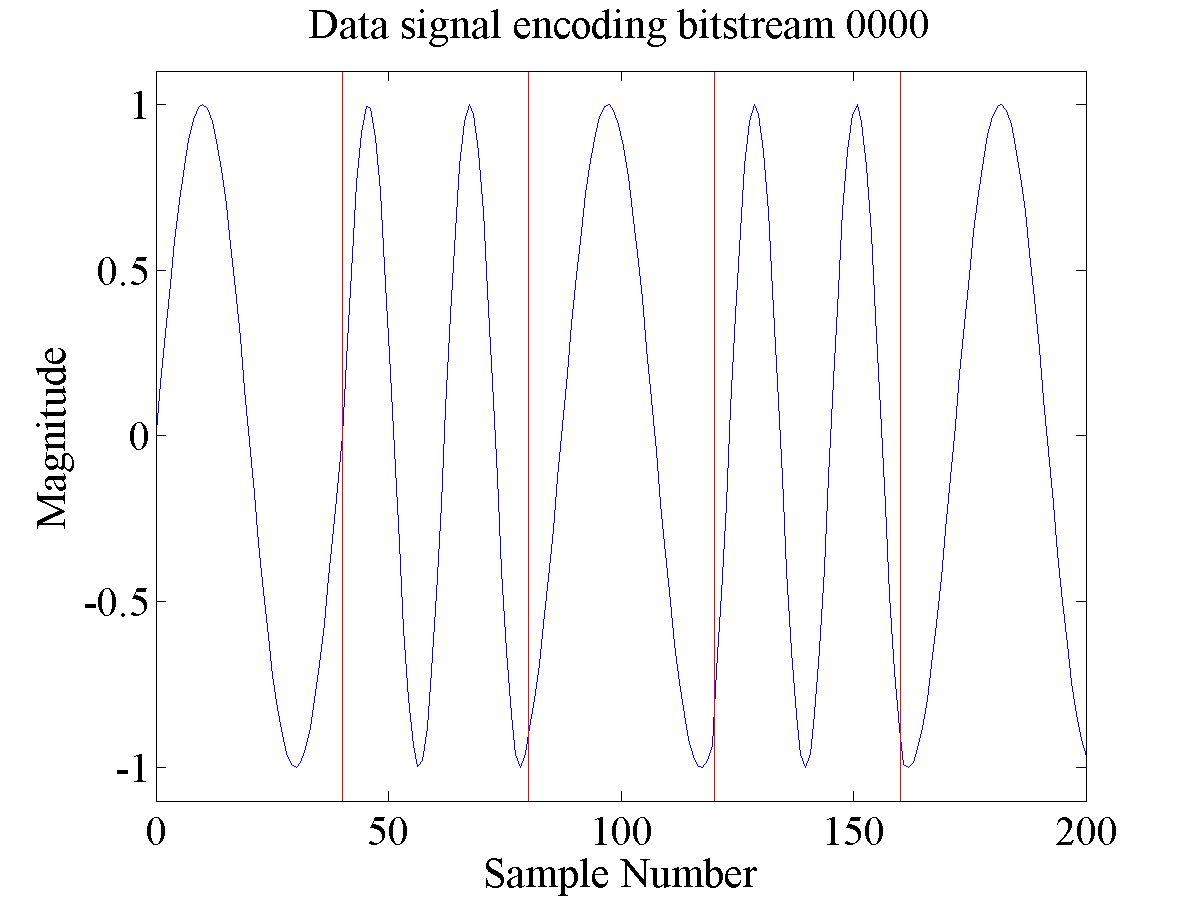
\includegraphics[width=0.75\linewidth]{images/Datasignalencodingbitstream0000.png} 
	\caption{Example Bell 202 signal encoding the bit stream '0000'.}
	\label{exampleBitStream}
\end{figure}
